% Figure from MATH 556 notes, section 10. Compile with the notes preamble.
\begin{tikzpicture}[scale=1.4, >=stealth]
    \draw[->, gray] (-1.4,0) -- (1.4,0);
    \draw[->, gray] (0,-1.4) -- (0,1.4);
    \draw[thick] (-1,-1) rectangle (1,1);
    \draw[thick, red!75!black] (0,0) circle (1);
    \draw[dashed] (-0.7071,-0.7071) rectangle (0.7071,0.7071);
    \node[anchor=west] at (1.08,1) {$\{\|x\|_\infty \le 1\}$};
    \draw[thin, red!75!black] (0.94,0.34) -- (1.08,0.34);
    \node[anchor=west, red!75!black] at (1.08,0.34) {$\{\|x\|_2 \le 1\}$};
    \draw[thin] (0.7071,-0.45) -- (1.08,-0.45);
    \node[anchor=west] at (1.08,-0.45) {$\{\|x\|_\infty \le \tfrac{1}{\sqrt{2}}\}$};
\end{tikzpicture}
